\documentclass[12pt]{extarticle}

\usepackage[utf8]{inputenc}
\usepackage{url}
\usepackage{graphicx}
\usepackage{amsmath}
\usepackage{hhline}
\usepackage{multicol}
\usepackage{float}
\usepackage{longtable}
\usepackage{geometry}
\usepackage[
    urldate=long,
    sorting=none
]{biblatex}
\addbibresource{mybib.bib}

\setlength{\tabcolsep}{0.5em} % for the horizontal padding
{\renewcommand{\arraystretch}{1.2}% for the vertical padding

\title{%
  Data Ethics Practical 3\\
  \vspace{5mm} 
  \large Data Protection Impact Assessment
  }

\author{\textit{Author}: 150008022}

\date{\today}


\begin{document}

\maketitle
\thispagestyle{empty}

\vfill
\begin{figure}[!ht]
    \centering
    
\includegraphics[width = 4.5cm]{images/standrewslogo.png}
\end{figure}
\vfill

\begin{quote}
    \centering
    \large{ "There is only one way at the end of the day to make technology better and that is to use it" 
    \par\emph{Brad Smith, Microsoft President, 2020}}
\end{quote}

\newpage
\pagenumbering{arabic}

\part{DPIA}

% In Step 1 you should describe your case study, and why it meets the requirements in Article 35(3).

\section*{Step 1: Identify the need for a DPIA} 

\begin{table}[H] 
\centering 
\begin{tabular}{p{\linewidth}} 
\hline %row no:1 
\multicolumn{1}{|p{\linewidth}|}{Explain broadly what project aims to achieve and what type of processing it involves. You may find it helpful to refer or link to other documents, such as a project proposal. Summarise why you identified the need for a DPIA.} \\ 
\hhline{-} %row no:2 
\end{tabular}
\end{table}
Microsofts' general purpose Face software can extract features such as age, emotion, gender, pose, smile, and facial hair from images of humans \cite{face}. 
Images can be cross referenced to determine if the same person appears in them, and emotions can be detected based on facial features.
West provides a compilation of current and future applications for facial recognition\cite{facefirst}, which range from unlocking mobile devices to identifying and finding missing children.

These features require an assessment of the impact of the envisaged processing operations on the protection of personal data, as they meet the requirement of Article 35(3)(a) \cite{EUdataregulations2018}: the facial recognition software attempts to profile individuals based on their appearance. The results of this profiling will likely be used to make decisions that affect the individual being profiled.

The project also requires a DPIA according to the UK ICO's guidance as it involves:
\begin{itemize}
    \itemsep0em 
    \item carrying out profiling on a large scale.
    \item processing of biometric data.
    \item process personal data that could result in a risk of physical harm in the event of a security breach.
\end{itemize}

\pagebreak

\section*{Step 2: Describe the processing} 

%%%%%%%%%%%%%%%%%%%% Table No: 3 starts here %%%%%%%%%%%%%%%%%%%% 
\begin{longtable}{p{\linewidth}} 
\hline %row no:1 
\multicolumn{1}{|p{\linewidth}|}{
\textbf{Describe the nature of the processing: }how will you collect, use, store and delete data? What is the source of the data? Will you be sharing data with anyone? You might find it useful to refer to a flow diagram or other way of describing data flows. What types of processing identified as likely high risk are involved?} \\*
\hhline{-} %row no:2 
\end{longtable} 

Figure \ref{fig:identify} shows an example of the facial recognition API usage flow for reference. The Face API processes three different categories of data \cite{robmazz}: 
\begin{itemize}
    \item Customer Data: any data provided by a customer using the service, such as images of faces and metadata attached to people and groups. 
          Usernames and billing information is also included in this category.
    \item Service Generated Data: logs and usage monitoring data which contains pseudonymized data. 
    \item Support Data: information provided by the customer when seeking technical support with the service. For example, emails asking how to use the service or how to resolve an issue.
\end{itemize}

% Collect
Consumers of the cognitive services API (Application Program Interface) provide custmer data which is used by the software. 
This includes images of people for identification and training. 
The URL of images are provided using HTTPS (Hypertext Transfer Protocol Secure), which are then fetched by the service to be processed. 
Service generated data is produced by the servers that process user requests. 
Support data is supplied by customers and the technical support team.

% Use
None of the images submitted are retained in their raw form. 
Instead, images are deconstructed on submission into face landmarks (coordinates of facial features) and attributes (age, emotion, gender, etc.) \cite{patrickfarley}. The face landmarks can be used to identify the same person appearing in different images, and for assessing their emotion or demographic. Users are also able to attach custom metadata to any group or person that they create using the API. 
Service generated data is used to determine billing of users, and for maintenance of the software.
Support data is used to identify usability issues with the software and help solve customer issues.

% Store
Processing and storage occurs in the cloud, specifically using Azure. 
Users can choose the geographical region that they would like their data to be stored. 
Data is stored using a multi-tenant approach, where multiple customers data will be stored on the same hardware \cite{terrylanfear}. 
However, the data is segregated such that users cannot access data they do not own.
Azure staff are unable to access the data without explicit permission from a user, and any access and is heavily monitored. 
Access to the data and model requires a cryptographic key. Two key types exist: an admin key which gives full rights to all operations and a query key which gives read-only access. Keys can be be created and revoked by users with the necessary permissions \cite{heidisteen}.

% Delete
The documentation shows that consumers of the API can delete anything they create (groups of people, individual people, face metadata) with immediate effect \cite{documentation}. 
When users delete data or remove their accounts, their data is destroyed by being overwritten. 
Physical hardware when decommissioned is also destroyed.

% Sharing
Customer data is not shared with any third parties, and is not accessible by default to Microsoft. 
This is achieved through access control, network security, and encryption of data at rest. 

% High Risk
Areas of high risk include the transit of data between user and the service, and the storage of the data and model. 
Data has the potential to be intercepted or accessed by an unauthorized entity at any of these stages.
Any logging of processes also has the potential to leak data. 
The preprocessing of the images to determine attributes such as gender also has a high level of risk. 
Both correct and incorrect classifications could influence individuals that are processed by the system. 

%%%%%%%%%%%%%%%%%%%% Table No: 3 ends here %%%%%%%%%%%%%%%%%%%% 

\begin{figure}[!ht]
    \centering
    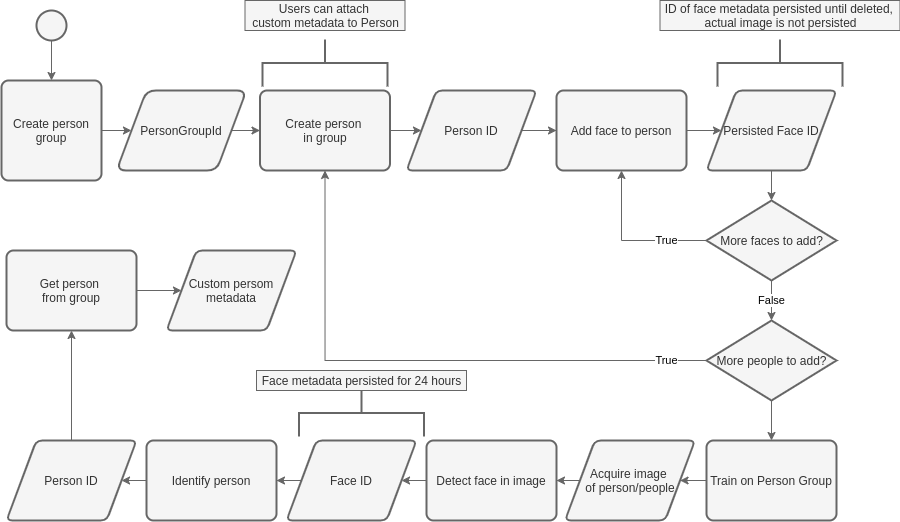
\includegraphics[width=\linewidth]{images/identifyflow}
    \caption{Usage flow for person identification} \label{fig:identify}
\end{figure}

%%%%%%%%%%%%%%%%%%%% Table No: 4 starts here %%%%%%%%%%%%%%%%%%%% 
\begin{table}[H] 
\centering 
\begin{tabular}{p{\linewidth}} 
\hline %row no:1 
\multicolumn{1}{|p{\linewidth}|}{
\textbf{Describe the scope of the processing: }what is the nature of the data, and does it include special category or criminal offence data? How much data will you be collecting and using? How often? How long will you keep it? How many individuals are affected? What geographical area does it cover?} \\ 
\hhline{-} %row no:2 
\end{tabular} 
\end{table} 

% Nature of the data
Customer data that will be processed includes raw images of faces that are supplied by the user, descriptions of faces detected by the service in these images as coordinates, generated categorisation data such as gender, emotions, and any metadata that the users tag groups/people/images with themselves. 


% Special category or criminal offence
Only the user supplied metadata is not essential to use the service. This data comes under GDPR special category data as it can be considered biometric data used to identify an individual.
Service generated data such as logs will likely contain the IP addresses of users and their usernames, which are considered personal data according to recital 30 of GPDR \cite{vollmer_2018} and by the UK ICO \cite{ico} respectively. 
Microsoft has no control over what data is stored under the user supplied metadata, ad so it is the responsibility of the user to determine appropriate use of this feature.

% How much data 
Each group can contain up to 1 million different person objects, and each person can have up to 248 faces registered \cite{faceoverview}. There is virtually no limit on the number of groups that users can create. 

% How often is data collected
Service generated data such as logs will be collected every time a user interacts with the service. 
Customer data is only collected when explicitly provided by the customer.

% How long is data kept
Processed face images for identification purposes are kept for 24 hours unless deleted by the user. Persisted faces used for model training are retained until deleted by the user.

% How many individuals are affected
The number of individuals affected corresponds to the the number of people and faces submitted to the service, as well as the number of users of the service. 
Both are potentially limitless.

% What geographical area does it cover
The Face API is available essentially worldwide. More details can be found at \cite{availability}.

%%%%%%%%%%%%%%%%%%%% Table No: 4 ends here %%%%%%%%%%%%%%%%%%%% 
\vspace{\baselineskip} 
%%%%%%%%%%%%%%%%%%%% Table No: 5 starts here %%%%%%%%%%%%%%%%%%%% 
\begin{table}[H] 
\centering 
\begin{tabular}{p{\linewidth}} 
\hline %row no:1 
\multicolumn{1}{|p{\linewidth}|}{
\textbf{Describe the context of the processing: }what is the nature of your relationship with the individuals? How much control will they have? Would they expect you to use their data in this way? Do they include children or other vulnerable groups? Are there prior concerns over this type of processing or security flaws? Is it novel in any way? What is the current state of technology in this area? Are there any current issues of public concern that you should factor in? Are you signed up to any approved code of conduct or certification scheme (once any have been approved)?} \\ 
\hhline{-} %row no:2 
\multicolumn{1}{|p{\linewidth}|}{
% TODO 
} \\ 
\hhline{-} 
\end{tabular} 
\end{table} 
%%%%%%%%%%%%%%%%%%%% Table No: 5 ends here %%%%%%%%%%%%%%%%%%%% 
\vspace{\baselineskip}
%%%%%%%%%%%%%%%%%%%% Table No: 6 starts here %%%%%%%%%%%%%%%%%%%%


\begin{table}[H]
 			\centering
\begin{tabular}{p{\linewidth}}
\hline
%row no:1
\multicolumn{1}{|p{\linewidth}|}{\textbf{Describe the purposes of the processing: }what\ do you want to achieve? What is the intended effect on individuals? What are the benefits of the processing – for  you, and more broadly? } \\
\hhline{-}
%row no:2
\multicolumn{1}{|p{\linewidth}|}{} \\
\hhline{-}

\end{tabular}
 \end{table}


%%%%%%%%%%%%%%%%%%%% Table No: 6 ends here %%%%%%%%%%%%%%%%%%%%

\section*{Step 3: Consultation process}
\addcontentsline{toc}{section}{Step 3: Consultation process}


%%%%%%%%%%%%%%%%%%%% Table No: 7 starts here %%%%%%%%%%%%%%%%%%%%


\begin{table}[H]
 			\centering
\begin{tabular}{p{\linewidth}}
\hline
%row no:1
\multicolumn{1}{|p{\linewidth}|}{\textbf{Consider how to consult with relevant stakeholders: }describe when and how you will seek individuals’ views – or justify why it’s not appropriate to do so. Who else do you need to involve within your organisation? Do you need to ask your processors to assist? Do you plan to consult information security experts, or any other experts?} \\
\hhline{-}
%row no:2
\multicolumn{1}{|p{\linewidth}|}{} \\
\hhline{-}

\end{tabular}
 \end{table}


%%%%%%%%%%%%%%%%%%%% Table No: 7 ends here %%%%%%%%%%%%%%%%%%%%


\vspace{\baselineskip}
\section*{Step 4: Assess necessity and proportionality}
\addcontentsline{toc}{section}{Step 4: Assess necessity and proportionality}


%%%%%%%%%%%%%%%%%%%% Table No: 8 starts here %%%%%%%%%%%%%%%%%%%%


\begin{table}[H]
 			\centering
\begin{tabular}{p{\linewidth}}
\hline
%row no:1
\multicolumn{1}{|p{\linewidth}|}{\textbf{Describe compliance and proportionality measures, in particular:} what is your lawful basis for processing? Does the processing actually achieve your purpose? Is there another way to achieve the same outcome? How will you prevent function creep? How will you ensure data quality and data minimisation? What information will you give individuals? How will you help to support their rights? What measures do you take to ensure processors comply? How do you safeguard any international transfers?} \\
\hhline{-}
%row no:2
\multicolumn{1}{|p{\linewidth}|}{} \\
\hhline{-}

\end{tabular}
 \end{table}


%%%%%%%%%%%%%%%%%%%% Table No: 8 ends here %%%%%%%%%%%%%%%%%%%%

\section*{Step 5: Identify and assess risks}
\addcontentsline{toc}{section}{Step 5: Identify and assess risks}


%%%%%%%%%%%%%%%%%%%% Table No: 9 starts here %%%%%%%%%%%%%%%%%%%%


\begin{table}[H]
\centering
\begin{tabular}{p{0.55\linewidth}p{0.15\linewidth}p{0.15\linewidth}p{0.15\linewidth}}
\hline
%row no:1
\multicolumn{1}{|p{0.55\linewidth}}{\textbf{Describe source of risk and nature of potential impact on individuals. }Include associated compliance and corporate risks\textbf{ }as necessary. } & 
\multicolumn{1}{|p{0.15\linewidth}}{{\fontsize{10pt}{12.0pt}\selectfont \textbf{Likelihood of harm}}} & 
\multicolumn{1}{|p{0.15\linewidth}}{{\fontsize{10pt}{12.0pt}\selectfont \textbf{Severity of harm}}} & 
\multicolumn{1}{|p{0.15\linewidth}|}{{\fontsize{10pt}{12.0pt}\selectfont \textbf{Overall risk }}} \\
\hhline{----}
%row no:2
\multicolumn{1}{|p{0.55\linewidth}}{} & 
\multicolumn{1}{|p{0.15\linewidth}}{{\fontsize{11pt}{13.2pt}\selectfont Remote, possible or probable}} & 
\multicolumn{1}{|p{0.15\linewidth}}{{\fontsize{11pt}{13.2pt}\selectfont Minimal, significant or severe}} & 
\multicolumn{1}{|p{0.15\linewidth}|}{{\fontsize{11pt}{13.2pt}\selectfont Low, medium or high}} \\
\hhline{----}

\end{tabular}
 \end{table}


%%%%%%%%%%%%%%%%%%%% Table No: 9 ends here %%%%%%%%%%%%%%%%%%%%

\section*{Step 6: Identify measures to reduce risk}
\addcontentsline{toc}{section}{Step 6: Identify measures to reduce risk}


%%%%%%%%%%%%%%%%%%%% Table No: 10 starts here %%%%%%%%%%%%%%%%%%%%


\begin{table}[H]
 			\centering
\begin{tabular}{p{0.99in}p{2.53in}p{0.83in}p{0.79in}p{0.79in}}
\hline
%row no:1
\multicolumn{5}{|p{\dimexpr\linewidth+8\tabcolsep\relax}|}{\textbf{Identify additional measures you could take to reduce or eliminate risks identified as medium or high risk in step 5}} \\
\hhline{-----}
%row no:2
\multicolumn{1}{|p{0.99in}}{\textbf{Risk }} & 
\multicolumn{1}{|p{2.53in}}{\textbf{Options to reduce or eliminate risk}} & 
\multicolumn{1}{|p{0.83in}}{\textbf{Effect on risk}} & 
\multicolumn{1}{|p{0.79in}}{\textbf{Residual risk}} & 
\multicolumn{1}{|p{0.79in}|}{\textbf{Measure approved}} \\
\hhline{-----}
%row no:3
\multicolumn{1}{|p{0.99in}}{} & 
\multicolumn{1}{|p{2.53in}}{} & 
\multicolumn{1}{|p{0.83in}}{Eliminated reduced accepted} & 
\multicolumn{1}{|p{0.79in}}{Low medium high} & 
\multicolumn{1}{|p{0.79in}|}{Yes/no} \\
\hhline{-----}

\end{tabular}
 \end{table}


%%%%%%%%%%%%%%%%%%%% Table No: 10 ends here %%%%%%%%%%%%%%%%%%%%


\vspace{\baselineskip}
\section*{Step 7: Sign off and record outcomes}
\addcontentsline{toc}{section}{Step 7: Sign off and record outcomes}


%%%%%%%%%%%%%%%%%%%% Table No: 11 starts here %%%%%%%%%%%%%%%%%%%%


\begin{table}[H]
 			\centering
\begin{tabular}{p{1.84in}p{2.16in}p{2.33in}}
\hline
%row no:1
\multicolumn{1}{|p{1.84in}}{\textbf{Item }} & 
\multicolumn{1}{|p{2.16in}}{\textbf{Name/position/date}} & 
\multicolumn{1}{|p{2.33in}|}{\textbf{Notes}} \\
\hhline{---}
%row no:2
\multicolumn{1}{|p{1.84in}}{Measures approved by:} & 
\multicolumn{1}{|p{2.16in}}{} & 
\multicolumn{1}{|p{2.33in}|}{{\fontsize{10pt}{12.0pt}\selectfont Integrate actions back into project plan, with date and responsibility for completion}} \\
\hhline{---}
%row no:3
\multicolumn{1}{|p{1.84in}}{Residual risks approved by:} & 
\multicolumn{1}{|p{2.16in}}{} & 
\multicolumn{1}{|p{2.33in}|}{{\fontsize{10pt}{12.0pt}\selectfont If accepting any residual high risk, consult the ICO before going ahead}} \\
\hhline{---}
%row no:4
\multicolumn{1}{|p{1.84in}}{DPO advice provided:} & 
\multicolumn{1}{|p{2.16in}}{} & 
\multicolumn{1}{|p{2.33in}|}{{\fontsize{10pt}{12.0pt}\selectfont DPO should advise on compliance, step 6 measures and whether processing can proceed}} \\
\hhline{---}
%row no:5
\multicolumn{3}{|p{\dimexpr\linewidth+4\tabcolsep\relax}|}{Summary of DPO advice:} \\
\hhline{---}
%row no:6
\multicolumn{1}{|p{1.84in}}{DPO advice accepted or overruled by:} & 
\multicolumn{1}{|p{2.16in}}{} & 
\multicolumn{1}{|p{2.33in}|}{{\fontsize{10pt}{12.0pt}\selectfont If overruled, you must explain your reasons}} \\
\hhline{---}
%row no:7
\multicolumn{3}{|p{\dimexpr\linewidth+4\tabcolsep\relax}|}{Comments:} \\
\hhline{---}
%row no:8
\multicolumn{1}{|p{1.84in}}{Consultation responses reviewed by:} & 
\multicolumn{1}{|p{2.16in}}{} & 
\multicolumn{1}{|p{2.33in}|}{{\fontsize{10pt}{12.0pt}\selectfont If your decision departs from individuals’ views, you must explain your reasons}} \\
\hhline{---}
%row no:9
\multicolumn{3}{|p{\dimexpr\linewidth+4\tabcolsep\relax}|}{Comments:} \\
\hhline{---}
%row no:10
\multicolumn{1}{|p{1.84in}}{This DPIA will kept under review by:} & 
\multicolumn{1}{|p{2.16in}}{} & 
\multicolumn{1}{|p{2.33in}|}{{\fontsize{10pt}{12.0pt}\selectfont The DPO should also review ongoing compliance with DPIA}} \\
\hhline{---}

\end{tabular}
 \end{table}
\part{Critical Assessment}

% what to do about general purpose storage solutions? 
% doesn't help draw the line between interconnected services (i.e. do I need to talk about the billing service here?)

\printbibliography

\end{document}

